\documentclass[12pt]{article}
\setlength{\textwidth}{17cm}
\setlength{\textheight}{24cm}
\setlength{\topmargin}{-2cm}
\setlength{\footskip}{1cm}
\setlength{\evensidemargin}{0cm}
\setlength{\oddsidemargin}{0cm}
\setlength{\parindent}{0cm}

\usepackage{allrunes}
\usepackage{amsmath}
\usepackage[english]{babel}
\usepackage[T1]{fontenc}
\usepackage[utf8]{inputenc}
\usepackage{fixltx2e}
\usepackage{multirow}

\usepackage[hyphens]{url}
\usepackage[unicode,colorlinks=true,breaklinks]{hyperref}
%\usepackage[dvips]{hyperref}
%should display links, but it does not work with \H accent
%and formulas in section titles

\hypersetup{colorlinks,linkcolor=blue,urlcolor=magenta,citecolor=magenta}
%Breaks long url`s in text, while keeping it one link:

\usepackage{amsfonts}
\usepackage{amsthm}
\usepackage{amssymb}


\theoremstyle{plain}
\usepackage{graphicx}

%\usepackage{gensymb}
\usepackage{float}

% For bra-ket notation
\usepackage{braket}

%% New commands
\newcommand{\dd}{\textrm{d}}

%% Pauli matrices
\newcommand{\sigx}{\sigma_x}
\newcommand{\sigy}{\sigma_y}
\newcommand{\sigz}{\sigma_z}

\newcommand{\paulix}{
    \left( \begin{array}{cc}
        0 & 1 \\
        1 & 0
    \end{array}
    \right)
}

\newcommand{\pauliy}{
    \left( \begin{array}{cc}
        0 & -i \\
        i & 0
    \end{array}
    \right)
}

\newcommand{\pauliz}{
    \left( \begin{array}{cc}
        1 & 0 \\
        0 & -1
    \end{array}
    \right)
}


\usepackage[bottom]{footmisc}

\begin{document}
\title{8th exam item}
\author{András Mátyás Biricz}

\maketitle


\newpage
\begin{abstract}
    Jelfeldolgozás és idősor-analízis – Fourier-módszerek, FFT, a spektrum és a spektrogram, az átviteli és ablakfüggvények, Wiener-szűrő. Korrelációs függvények, a Wiener–Hin-csin-tétel és a teljesítményspektrum. Konvolúció és dekonvolúció. Szűrők analóg és digitális megvalósítása, RLC-körök, FIR- és IIR-szűrők.

	Signal processing and analysis of time series - Fourier methods, FFT, spectrum and spectrogram, transfer- and window functions, Wiener-filter. Correlation functions, Wiener-Khinchin theorem, power spectrum. Convolution, deconvolution. Realization of analog and digital filters, RLC-circuit, FIR and IIR filters. 

\end{abstract}

\section{Introduction}

Signal processing is a subfield of electrical engineering that concerns the analysis, synthesis, and modification of signals\footnote{\url{https://en.wikipedia.org/wiki/Signal_processing}.} in order to extract information of phenomena through processing of audio, video and the outcome of various measurements. Signal processing techniques can be used to improve signal transmission, emphasize or detect interesting components of measured signal and to improve storage efficiency. 

As a consequence of the technological advancement tremendous amount of data can be measured in various fields of science and it becomes even bigger challenge to deal with that vast amount of data. Fortunately, the application of the signal processing methods can help.

\section{Fourier methods}

Fourier methods play a key role in analysing signals, especially in case of time series data. These methods involve the Fourier-series and Fourier transform. As a result we can acquire valuable information as a (frequency) spectrum. In addition, these can be applicable more broadly, even to analyse spatial properties of 2 or 3 dimensional signals or to solve differential equations. Last but not least, it comes in handy in calculation of correlation and convolution.

\subsection{Fourier series}

A Fourier series is an expansion of a periodic function $f(x)$ in terms of an infinite sum of sines and cosines. Fourier series make use of the orthogonality relationships of the sine and cosine functions. The computation and study of Fourier series is known as harmonic analysis and is extremely useful as a way to break up an arbitrary periodic function into a set of simple terms that can be plugged in, solved individually, and then recombined to obtain the solution to the original problem or an approximation to it to whatever accuracy is desired or practical. 

In particular, since the superposition principle holds for solutions of a linear homogeneous ordinary differential equation, if such an equation can be solved in the case of a single sinusoid, the solution for an arbitrary function is immediately available by expressing the original function as a Fourier series and then plugging in the solution for each sinusoidal component. In some special cases where the Fourier series can be summed in closed form, this technique can even yield analytic solutions.

In addition, any set of functions that form a complete orthogonal system has a corresponding generalized Fourier series analogous to the Fourier series. For example, using orthogonality of the roots of a Bessel function of the first kind gives a so-called Fourier-Bessel series.

The computation of the Fourier series is based on integral identities (follow source link to view). For a $2 \pi$ periodic function $f(x)$, the series expansion is the following:

\begin{equation}
f(x) = \frac{1}{2} a_0 + \sum_{n=1}^{\infty} a_n cos(n x) + \sum_{n=1}^{\infty} b_n sin(n x),
\end{equation}
where 

\begin{equation}
a_0 = \frac{1}{\pi} \int_{-\pi}^{\pi} f(x) \text{d}x,
\end{equation}

\begin{equation}
a_n = \frac{1}{\pi} \int_{-\pi}^{\pi} f(x) cos(nx) \text{d}x,
\end{equation}

\begin{equation}
b_n = \frac{1}{\pi} \int_{-\pi}^{\pi} f(x) sin(nx) \text{d}x,
\end{equation}
where $a_0$ is the coefficient of the constant term, $a_n$ and $b_n$ are the coefficients of the periodic terms and $n=1,2,3, ...$.

The notion of a Fourier series can also be extended to complex coefficients. In case of a real-valued function $f(x)$:

\begin{equation}
f(x) = \sum_{n=-\infty}^{\infty} A_n e^{i n x}.
\end{equation}

It can be showed (follow source), that:

\begin{equation}
A_n = \frac{1}{2 \pi} \int_{-\pi}^{\pi} f(x) e^{-i n x} \text{d}x,
\end{equation}
which are coefficients hiding the $a_0$, $a_n$, $b_n$ coefficients in a compact form.

Note, that not only $2 \pi$ periodic functions can be expanded in a Fourier series, it can be generalized to the case of a function periodic in $[-L/2, L/2]$:

\begin{equation}
f(x) = \sum_{n=-\infty}^{\infty} A_n e^{i 2 \pi n x/L},
\end{equation}

\begin{equation}
A_n = \frac{1}{L} \int_{-L/2}^{L/2} f(x) e^{i 2 \pi n x/L} \text{d}x.
\end{equation}

The source and more information with examples can be found by following this link\footnote{\url{http://mathworld.wolfram.com/FourierSeries.html}}. 

\subsection{Fourier transform}

The Fourier transform is a generalization of the complex Fourier series in the limit as $L \rightarrow	\infty$. Replace the discrete $A_n$ with the continuous $F(k)dk$ while letting  $n/L \rightarrow k$. Then change the sum to an integral, and the equations become:

\begin{equation}
f(x) = \int_{-\infty}^{\infty} F(k) e^{i 2 \pi k x} \text{d}k,
\end{equation}

\begin{equation}
f(k) = \int_{-\infty}^{\infty} f(x) e^{-i 2 \pi k x} \text{d}x.
\end{equation}

Note that some authors (especially physicists) prefer to write the transform in terms of angular frequency $\omega \equiv 2 \pi \nu$) instead of the oscillation frequency ($\nu$). However, this destroys the symmetry, resulting in the transform pair:


\begin{equation}
H(\omega) = \mathcal{F}[h(t)] = \int_{-\infty}^{\infty} h(t) e^{-i \omega t} \text{d}t,
\end{equation}

\begin{equation}
h(t) = \mathcal{F}^{-1}[H(\omega)] = \frac{1}{2 \pi} \int_{-\infty}^{\infty} H(\omega) e^{i \omega t} \text{d}\omega.
\end{equation}

A function $f(x)$ has a forward and inverse Fourier transform if:

\begin{itemize}
	\item $\int_{-\infty}^{\infty} |f(x)| \text{d}x$ exists,
	\item there are a finite number of discontinuities,
	\item the function has bounded variation. (A sufficient weaker condition is fulfillment of the Lipschitz condition.\footnote{\url{http://mathworld.wolfram.com/LipschitzCondition.html}.})
\end{itemize}

The Fourier transform is linear, which means the following for functions $f(x)$ and $g(x)$:

\begin{equation}
\mathcal{F}[a f(x) + b g(x)] = a \mathcal{F}[f(x)] + b \mathcal{F}[g(x)] = a F(k) + b G(k).
\end{equation}

The source and more information with examples can be found by following this link\footnote{\url{http://mathworld.wolfram.com/FourierTransform.html}}. 

\subsection{Fast Fourier Transform}

A fast Fourier transform (FFT) is an algorithm that computes the discrete Fourier transform (DFT) of a sequence, or its inverse (IDFT). The DFT is obtained by decomposing a sequence of values into components of different frequencies. This operation is useful in many fields, but computing it directly from the definition is often too slow to be practical. An FFT rapidly computes such transformations by factorizing the DFT matrix into a product of sparse (mostly zero) factors. As a result, it manages to reduce the complexity of computing the DFT from $\mathcal{O}(N^{2})$, which arises if one simply applies the definition of DFT, to $\mathcal{O}(N log N)$, where $N$ is the data size. The difference in speed can be enormous, especially for long data sets where $N$ may be in the thousands or millions. In the presence of round-off error, many FFT algorithms are much more accurate than evaluating the DFT definition directly. There are many different FFT algorithms based on a wide range of published theories, from simple complex-number arithmetic to group theory and number theory.\footnote{\url{https://en.wikipedia.org/wiki/Fast_Fourier_transform}.}

Let $x_0$, ..., $x_{N-1}$ be complex numbers. The DFT is defined by the formula:

\begin{equation}
X_k = \sum_{n=0}^{N-1} x_n e^{-i2\pi k n/N}, ~~~ k = 0, \ldots, N-1,
\end{equation}
where $e^{i 2\pi/N}$ is a primitive $N^{\text{th}}$ root of 1.

Evaluating this definition directly requires $\mathcal{O}(N^2)$ operations: there are $N$ outputs $X_k$, and each output requires a sum of $N$ terms. An FFT is any method to compute the same results in $\mathcal{O}(N log N)$ operations. All known FFT algorithms require $\mathcal{O}(N log N)$ operations, although there is no known proof that a lower complexity score is impossible.

To illustrate the savings of an FFT, consider the count of complex multiplications and additions for $N=4096$ data points. Evaluating the DFT's sums directly involves $N^2$ complex multiplications and $N(N-1)$ complex additions, of which $\mathcal{O}(N)$ operations can be saved by eliminating trivial operations such as multiplications by 1. On the other hand, the Radix-2 (\hyperlink{James W. Cooley and John W. Tukey (1965)}{James W. Cooley and John W. Tukey (1965)}) algorithm, for $N$ a power of 2, can compute the same result with only $N/2 log_2 N$ complex multiplications (again, ignoring simplifications of multiplications by 1 and similar) and $N log_2 N$ complex additions. In practice, actual performance on modern computers is usually dominated by factors other than the speed of arithmetic operations and the analysis is a complicated subject, but the overall improvement from $\mathcal{O}(N^2)$ to $\mathcal{O} (N log N)$ remains.


A Radix-2 decimation-in-time (DIT) FFT is the simplest and most common form of the Cooley–Tukey algorithm, although highly optimized Cooley–Tukey implementations typically use other forms of the algorithm as described below. Radix-2 DIT divides a DFT of size $N$ into two interleaved DFTs (hence the name "Radix-2") of size $N/2$ with each recursive stage.

The discrete Fourier transform (DFT) is defined by the formula:

\begin{equation}
X_k = \sum_{n=0}^{N-1} x_n e^{-\frac{2\pi i}{N} nk},
\end{equation}
where $k$ is an integer ranging from $0$ to $N-1$.

Radix-2 DIT first computes the DFTs of the even-indexed inputs
$(x_{2m}=x_0, x_2, \ldots, x_{N-2})$ and of the odd-indexed inputs $(x_{2m+1}=x_1, x_3, \ldots, x_{N-1})$, and then combines those two results to produce the DFT of the whole sequence. This idea can then be performed recursively to reduce the overall runtime to $\mathcal{O}(N log N)$. This simplified form assumes that $N$ is a power of two, since the number of sample points $N$ can usually be chosen freely by the application (e.g. by changing the sample rate or window, zero-padding, etcetera), this is often not an important restriction.

The Radix-2 DIT algorithm rearranges the DFT of the function $x_n$ into two parts: a sum over the even-numbered indices ($n={2m}$) and a sum over the odd-numbered indices ($n={2m+1}$):

\begin{equation}
\begin{matrix} X_k & =
& \sum \limits_{m=0}^{N/2-1} x_{2m}e^{-\frac{2\pi i}{N} (2m)k}   +   \sum \limits_{m=0}^{N/2-1} x_{2m+1} e^{-\frac{2\pi i}{N} (2m+1)k}
  \end{matrix}.
\end{equation}

One can factor a common multiplier $e^{-\frac{2\pi i}{N}k}$ out of the second sum, as shown in the equation below. It is then clear that the two sums are the DFT of the even-indexed part $x_{2m}$ and the DFT of odd-indexed part $x_{2m+1}$ of the function $x_n$. Denote the DFT of the even-indexed inputs $x_{2m}$ by $E_k$ and the DFT of the odd-indexed inputs $x_{2m + 1}$ by $O_k$ and we obtain:

\begin{equation}
\begin{matrix} X_k= \underbrace{\sum \limits_{m=0}^{N/2-1} x_{2m}   e^{-\frac{2\pi i}{N/2} mk}}_{\mathrm{DFT\;of\;even-indexed\;part\;of\;} x_n} {} +  e^{-\frac{2\pi i}{N}k}
 \underbrace{\sum \limits_{m=0}^{N/2-1} x_{2m+1} e^{-\frac{2\pi i}{N/2} mk}}_{\mathrm{DFT\;of\;odd-indexed\;part\;of\;} x_n} =  E_k + e^{-\frac{2\pi i}{N}k} O_k.
\end{matrix}
\end{equation}

Thanks to the periodicity of the complex exponentials, $X_{k+\frac{N}{2}}$ is also obtained from $E_k$ and $O_k$:

\begin{equation}
\begin{split}
X_{k + \frac{N}{2}} =  \sum \limits_{m=0}^{N/2-1} x_{2m} e^{-\frac{2\pi i}{N/2} m(k + \frac{N}{2})} +  e^{-\frac{2\pi i}{N}(k + \frac{N}{2})} \sum \limits_{m=0}^{N/2-1} x_{2m+1} e^{-\frac{2\pi i}{N/2} m(k + \frac{N}{2} )} \\  =  \sum \limits_{m=0}^{N/2-1} x_{2m}   e^{-\frac{2\pi i}{N/2} mk} e^{-2\pi m i} +  e^{-\frac{2\pi i}{N}k}e^{-\pi i} \sum \limits_{m=0}^{N/2-1} x_{2m+1} e^{-\frac{2\pi i}{N/2} mk} e^{-2\pi m i} \\ =  \sum \limits_{m=0}^{N/2-1} x_{2m}  e^{-\frac{2\pi i}{N/2} mk} - e^{-\frac{2\pi i}{N}k} \sum \limits_{m=0}^{N/2-1} x_{2m+1} e^{-\frac{2\pi i}{N/2} mk} \\ =  E_k - e^{-\frac{2\pi i}{N}k} O_k.
\end{split}
\end{equation}

We can rewrite $X_k$ as:

\begin{equation}
\begin{matrix}
X_k & =
& E_k + e^{-\frac{2\pi i}{N}k} O_k, \\
X_{k+\frac{N}{2}} & =
& E_k - e^{-\frac{2\pi i}{N}{k}} O_k.
\end{matrix}
\end{equation}

This result, expressing the DFT of length $N$ recursively in terms of two DFTs of size $N/2$, is the core of the Radix-2 DIT fast Fourier transform. The algorithm gains its speed by re-using the results of intermediate computations to compute multiple DFT outputs.  Note that final outputs are obtained by a $\pm$ combination of $E_k$ and $O_k \exp(-2\pi i k/N)$, which is simply a size-2 DFT (sometimes called a butterfly diagram in this context (see figure \ref{radix_fig})); when this is generalized to larger radices, the size-2 DFT is replaced by a larger DFT (which itself can be evaluated with an FFT).

The source and more information with examples can be found by following these links\footnote{\url{https://en.wikipedia.org/wiki/Cooley\%E2\%80\%93Tukey_FFT_algorithm},}\footnote{\url{https://en.wikipedia.org/wiki/Fast_Fourier_transform}.}.

\begin{figure}[h!]
    \centering
	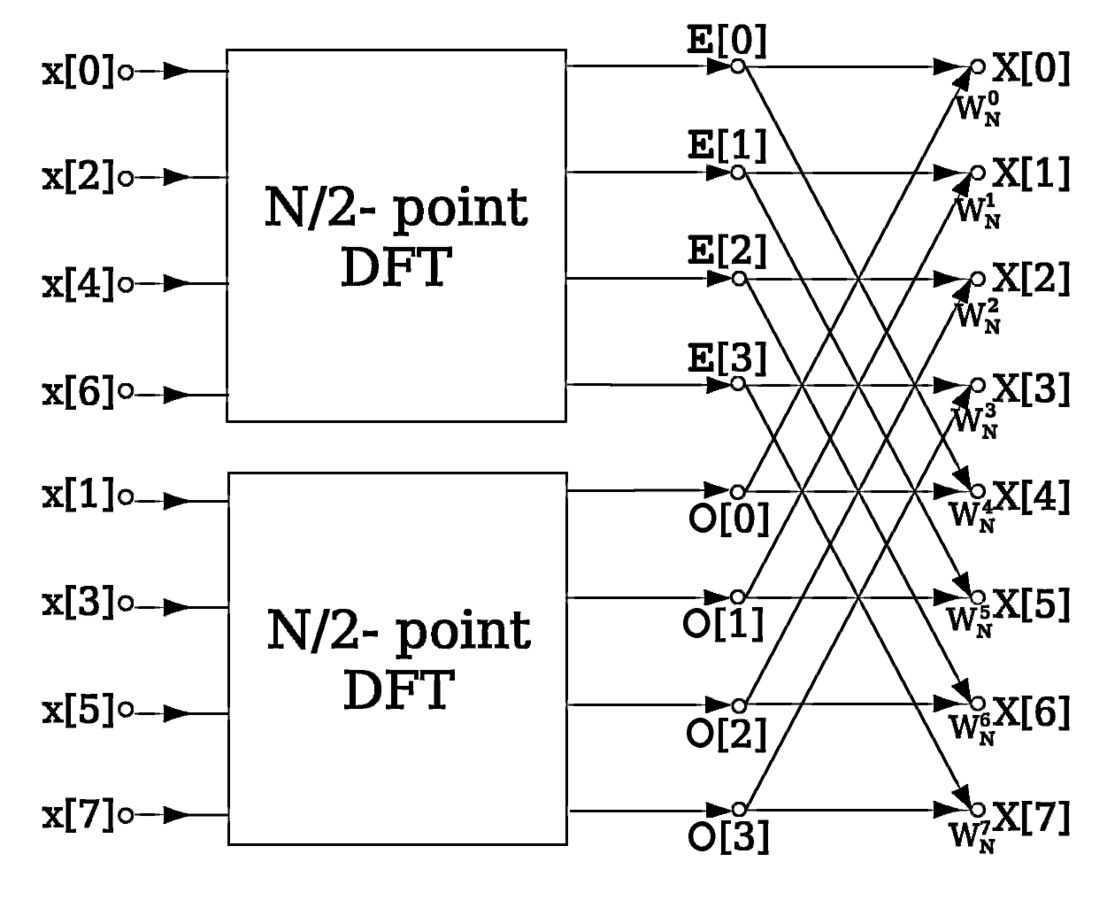
\includegraphics[width=.7\linewidth]{media/DIT-FFT-butterfly.png}
	\caption{Data flow diagram for $N=8$: a decimation-in-time radix-2 FFT breaks a length-$N$ DFT into two length-$N/2$ DFTs followed by a combining stage consisting of many size-2 DFTs called "butterfly" operations (so-called because of the shape of the data-flow diagrams). The source was accessed in June 2019 (\url{https://en.wikipedia.org/wiki/File:DIT-FFT-butterfly.png}).}
	\label{radix_fig}
\end{figure}

\subsection{Spectrum, spectrogram}

The spectrum is the (frequency) domain representation of a signal. A spectrogram is a visual representation of the spectrum of frequencies of a signal as it varies with time (see figures \ref{spectrogram_1} and \ref{spectrogram_2}). When applied to an audio signal, spectrograms are sometimes called sonographs, voiceprints, or voicegrams. When the data is represented in a 3D plot they may be called waterfalls. Spectrograms are used extensively in the fields of music, sonar, radar, and speech processing, seismology, and others. Spectrograms of audio can be used to identify spoken words phonetically, and to analyse the various calls of animals.

\begin{figure}[h!]
    \centering
	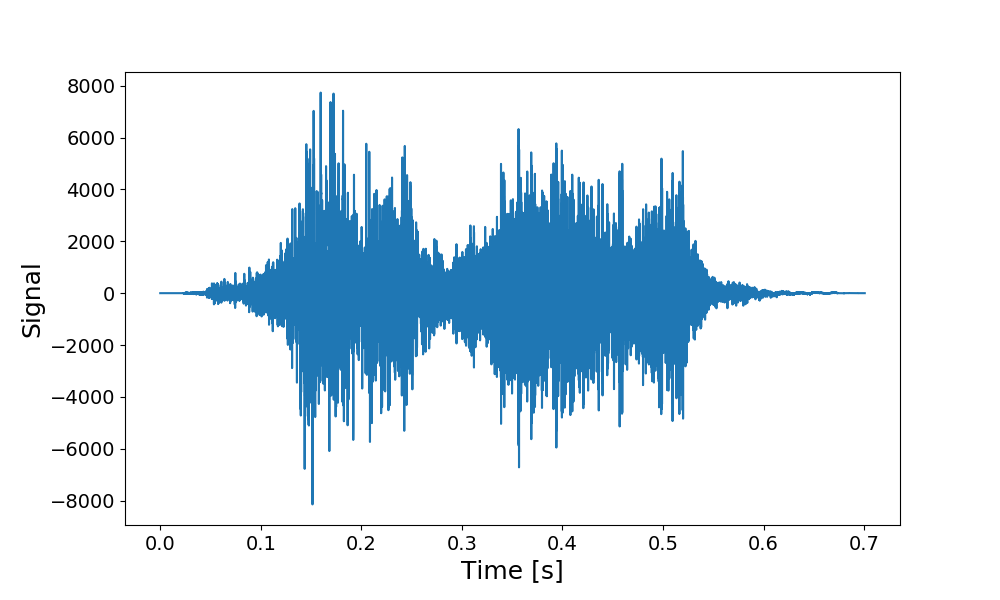
\includegraphics[width=.9\linewidth]{media/yes_sound_time.png}
	\caption{Yes sound. Source: \url{https://www.pacdv.com/sounds/voices/yes-2.wav}.}
	\label{spectrogram_1}
\end{figure}

\begin{figure}[h!]
    \centering
	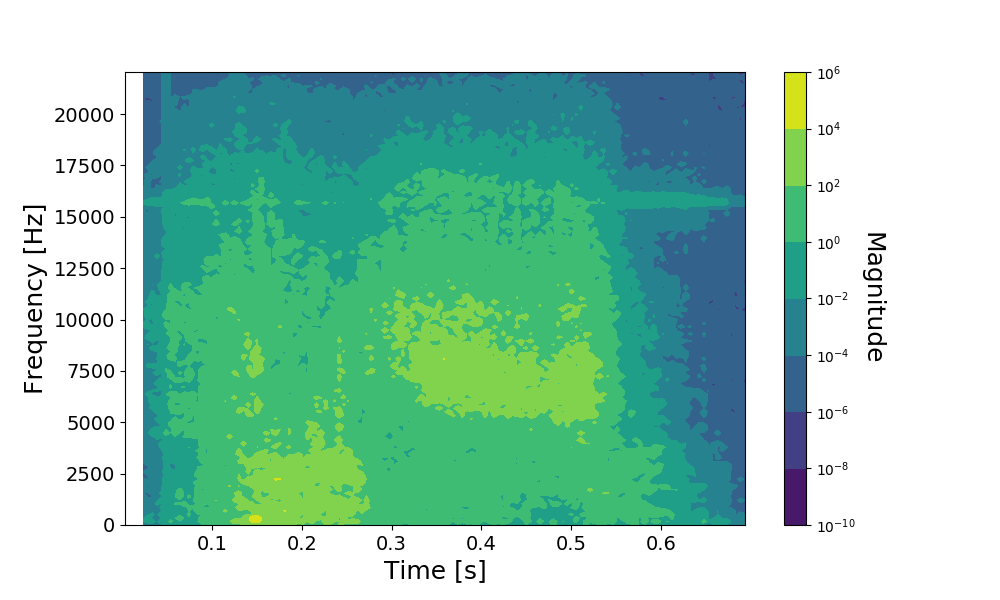
\includegraphics[width=.9\linewidth]{media/yes_sound_spectrogram.png}
	\caption{Spectrogram of the yes sound.}
	\label{spectrogram_2}
\end{figure}

%/media/abiricz/Storage/ELTE/Fizika9félév/Data mining and machine learning/lab10/yes_sound_spectrogram.png
%/media/abiricz/Storage/ELTE/Fizika9félév/Data mining and machine learning/lab10/yes_sound_time.png



\section{Correlation functions}



\section{Convolution}


\section{Transfer and window functions}


\section{Filters}


\subsection{Analog}


\subsection{Digital}


\subsection{RLC circuit}


\subsection{FIR}


\subsection{IIR}


\subsection{Wiener-filter}



\section{Conclusion}

\newpage
\begin{thebibliography}{Nature}
%\bibliography{references}

\bibitem{James W. Cooley and John W. Tukey (1965)}\hypertarget{James W. Cooley and John W. Tukey (1965)}{}
James W. Cooley and John W. Tukey. An Algorithm for the Machine Calculation of Complex Fourier Series \textit{Math. Comp.} \textbf{19} (1965), 297-301. \url{https://www.ams.org/journals/mcom/1965-19-090/S0025-5718-1965-0178586-1/S0025-5718-1965-0178586-1.pdf}

\end{thebibliography}




\end{document}
